\documentclass[a4paper,12pt,english]{all-in-one} %% TWOSIDE
\usepackage{ebgaramond}
\usepackage{amsmath} 
\usepackage{newtxmath}
\usepackage{multicol}
\usepackage{lipsum}
\usepackage{subfig}
\usepackage{listings}
\usepackage[hidelinks]{hyperref}
\newcommand\tab[1][1cm]{\hspace*{#1}} 
\newtagform{noparen}{}{}
\usetagform{noparen}

\doctitle{Modern Physics Laboratory }
\docsubtitle{X-ray Bragg Diffraction} % Experiment name here

\makeatletter
\title{{\large\textit{Modern Physics Laboratory | PHYS-461}}\\[0.5cm]{\Huge\color{gray}\textsc{\@docsubtitle}}}
\makeatother

\author{\textbf{Cordney Nash}  \and Micah Hillman  }
\date{September 30, 2024}
\footext{}



\begin{document}

\begin{titlepage}
\maketitle\vfill
\end{titlepage}
\newpage


\section*{Introduction}
{
\tab This experiment explores the constructive diffraction of X-rays incidented on Lithium Fluoride (LiF), Sodium chloride (NaCl) crystals and powdered crystalline samples. The resulting diffraction patterns show sharp maxima at specific angles, which are dependent on the wavelength of the X-rays and the crystal structure. A Geiger-Müller tube is used to detect and measure the diffracted X-rays as a function of the scattering angle. From here different properties of the crystal can be determined, such as the distance between successive planes.
}

\begin{figure}[h!]
    \centering
    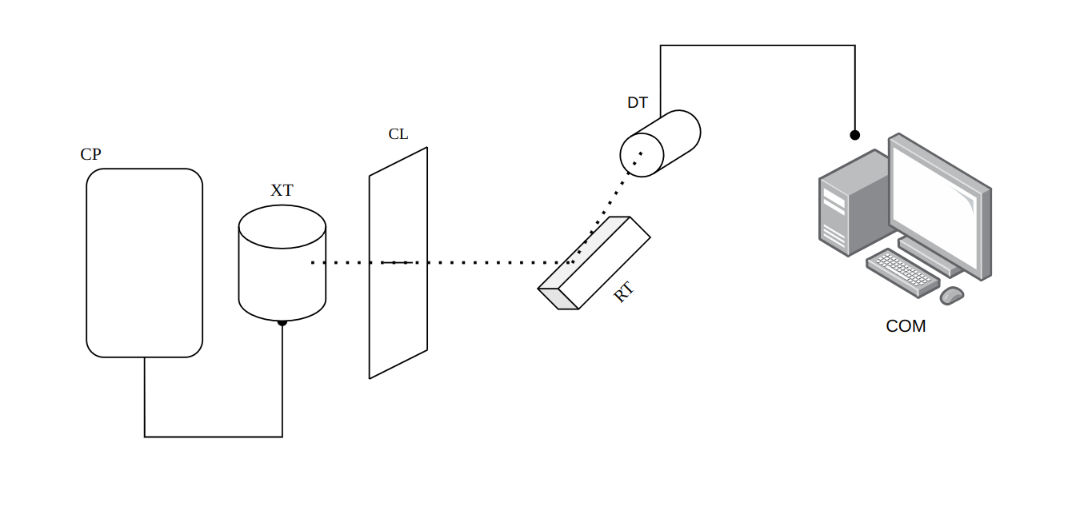
\includegraphics[width=0.8\linewidth]{3-xray/overleaf/Images/xray_diagram.png}
    \caption{ \scriptsize{ Control Panel (CP), Copper X-ray Tube (XT), Collimation Wall (CL), Rotating Table (RT), Detector Tube (DT), Computer (COM).
    } }
    \label{fig:enter-label}
\end{figure}

\begin{multicols}{2}

\section*{Theory \& Procedure}
{
\tab When stimulated, a copper anode emits two distinct characteristic X-rays: $K_\alpha$ and $K_\beta$. The $K_\alpha$ radiation, with a wavelength of 1.542 Å, occurs when an electron transitions from the $n=2$ shell to a vacant $n=1$ shell. In contrast, the $K_\beta$ radiation, with a wavelength of 1.392 Å, arises when an electron transitions from the $n=3$ shell to a vacant $n=1$ shell.

Given the extremely short wavelengths of X-rays, it is evident that a diffraction grating on the order of atomic dimensions is necessary to analyze the outgoing radiation effectively. To achieve this, we utilized LiF and NaCl crystals, along with a powdered LiF sample.

Crystalline materials have a periodic atomic structure that forms a lattice. In this lattice arrangement, when light is reflected from successive atomic planes, constructive interference occurs according to Bragg's Law, as described by Eq.\eqref{eq:1}. However, some of the X-ray's energy can continue to travel through the crystal.
\begin{equation}\label{eq:1}
    n\lambda = 2dsin\theta
\end{equation}
Where $d$ is the spacing between planes, $\theta$ is the angle the light is reflected back relative to the plane, n is the order of diffraction, and $\lambda$ is the wavelength.
(ADD more theory)

To begin the experiment, we powered the Leybold Didactic (LD) X-ray apparatus. This apparatus holds 3 different sections: (1) the control panel, used to adjust experimental parameters, (2) the X-ray tube housing a copper anode, and (3) a Geiger-Müller detector positioned with the experimental sample. The apparatus also features lead glass shielding which controlls the voltage switch (to the copper anode), allowing visibility while ensuring protection from X-ray exposure. Additionally, this whole device is connected to a computer where we can externally control starting parameters. 

For the measurements, we placed the desired sample on a rotating stage, which rotates at an angle of 2$\theta$ relative to the detector’s movement. Initial measurements were taken with the two crystal samples, which took approximately 15 minutes each. The powdered sample, due to its powdered nature, required around 3 hours for viable measurements. Before each run, we reset the system to ensure the starting angle was calibrated at $\theta$ = 0. From here, we set our starting parameters, and started measuring.  
}
    
\section*{Analysis \& Results}
{
When analyzing the diffraction data for crystals you first notice that each peak occurs in pairs, with the less intense peak consistently corresponding to $K_\beta$. Each pair after should be understood as a increase in the order of diffraction. By utilizing the measured angle $\theta$, the diffraction order, and the known wavelength $\lambda$, we can apply Eq.\eqref{eq:1} to calculate the plane spacing $d$. From this, the lattice constant can be determined with $2d$.



% \begin{table*}[]
% \parbox{.40\linewidth}{
% % \centering
% \begin{tabular}{l|r|r|r|r|r}
% peak \# & angle ($^\circ$) & n & X-ray, $\lambda$ & $d$ & $a_0$ \\ \hline
% 1 & 19 & 1 & $K_\beta$ & 2.14E-10 & 4.28E-10  \\
% 2 & 23 & 1 & $K_\alpha$ & 1.97E-10 & 3.95E-10 \\
% 3 & 44 & 2 & $K_\beta$ & 9.67E-11	& 1.93E-10\\
% 4 & 49 & 2 & $K_\alpha$ & 1.16E-10 & 2.33E-10 \\   
% \end{tabular}
% \caption{Crystalline information for the LiF sample \label{LiF}}
% }
% \hfill
% \parbox{.45\linewidth}{
% \centering
% \begin{tabular}{l|r|r|r|r|r}
% peak \# & angle ($^\circ$) & n & X-ray, $\lambda$ & $d$ & $a_0$ \\ \hline
% 1 & 14 & 1 & $K_\beta$ & 2.88E-10 & 5.75E-10  \\
% 2 & 16 & 1 & $K_\alpha$ & 2.80E-10 & 5.59E-10 \\
% 3 & 29 & 2 & $K_\beta$ & 2.87E-10 & 5.74E-10\\
% 4 & 33 & 2 & $K_\alpha$ & 2.83E-10 & 5.66E-10 \\  
% \end{tabular}
% \caption{Crystalline information for the NaCl sample.t \label{NaCl}}
% }
% \end{table*}

The results from the LiF and NaCl crystal, can be seen in Table \ref{tab:lif} and \ref{tab:nacl}. The accepted lattice constant is 4.05 {\AA} and 5.68 {\AA} for LiF and NaCl respectfully. Our measured lattice constant for Nacl is exactly the same as the accepted value, but for LiF this measured value is not same. We suspect one of the systematic errors that may have caused this is that the sample may not have been as smooth as it needed to be. This could cause the x-rays to interact with the atoms in complicated ways at the surface. 


}


\end{multicols}

\section*{Summary}
{
In conclusion, this experiment demonstrated the principles of constructive X-ray diffraction on crystals and powdered crystalline samples. By using a copper anode to emit characteristic X-rays and a sophisticated detector, we observed distinct diffraction patterns. These patterns, governed by Bragg’s Law, allowed us to calculate key crystal properties such as the spacing between atomic planes and the lattice constant. These patterns also allowed us to gain a better understanding of how Miller Indices can describe the interaction X-rays have with different planes with varying orientations. In all this experiment provided valuable insights into crystal structure and how X-rays scatter based on the arrangement and orientation of crystalline planes.
}

\begin{table*}[htb]
\centering
\begin{tabular}{c|c|c|c|c|c|c|c}
peak \# & angle ($^\circ$) & n & X-ray, $\lambda$ (m) & $d$ (m) & $a_0$ (m) & $\overline{a_0}$ (m) & $\overline{a_0}$ (\AA) \\ \hline
1 & 19 & 1 & $K_\beta$ & 2.14E-10 & 4.28E-10  & 3.12E-10 & 3.12\\
2 & 23 & 1 & $K_\alpha$ & 1.97E-10 & 3.95E-10 \\
3 & 44 & 2 & $K_\beta$ & 9.67E-11	& 1.93E-10\\
4 & 49 & 2 & $K_\alpha$ & 1.16E-10 & 2.33E-10 \\   
\end{tabular}
\caption{Crystalline information for the LiF crystal. }
\label{tab:lif}
\end{table*}

\begin{table*}[htb]
\centering
\begin{tabular}{c|c|c|c|c|c|c|c|c}
peak \# & angle ($^\circ$) & n & X-ray, $\lambda$ (m) & $d$ (m) & $a_0$ (m) & $\overline{a_0}$ (m) & $\overline{a_0}$ (\AA) \\ \hline
1 & 14 & 1 & $K_\beta$ & 2.88E-10 & 5.75E-10 & 5.68E-10 & 5.68 \\
2 & 16 & 1 & $K_\alpha$ & 2.80E-10 & 5.59E-10 \\
3 & 29 & 2 & $K_\beta$ & 2.87E-10 & 5.74E-10\\
4 & 33 & 2 & $K_\alpha$ & 2.83E-10 & 5.66E-10 \\  
\end{tabular}
\caption{Crystalline information for the NaCl crystal.}
\label{tab:nacl}
\end{table*}



\end{document}